\documentclass[11pt,a4paper]{article}

\usepackage[left=1.0in,right=1.0in,top=1.0in,bottom=1.0in,headheight=14pt,headsep=10pt,footskip=20pt]{geometry}
\usepackage{amsmath}
\usepackage{amssymb}
\usepackage{graphicx}
\usepackage{booktabs}
\usepackage{array}
\usepackage{multirow}
\usepackage{xcolor}
\usepackage{setspace}
\usepackage{hyperref}
\usepackage{fancyhdr}
\usepackage{algorithm}
\usepackage{algpseudocode}
\usepackage{caption}
\usepackage{subcaption}
\usepackage{float}
\usepackage{titlesec}

\setstretch{1.2}
\setlength{\parskip}{5pt}
\setlength{\parindent}{0pt}

% Consistent, moderate heading sizes
\titleformat{\section}{\normalfont\large\bfseries}{\thesection}{0.7em}{}
\titleformat{\subsection}{\normalfont\normalsize\bfseries}{\thesubsection}{0.7em}{}
\titleformat{\subsubsection}{\normalfont\normalsize\itshape}{\thesubsubsection}{0.7em}{}
\titlespacing*{\section}{0pt}{10pt}{6pt}
\titlespacing*{\subsection}{0pt}{8pt}{4pt}
\titlespacing*{\subsubsection}{0pt}{6pt}{3pt}

\pagestyle{fancy}
\fancyhf{}
\lhead{Fairness in Federated Learning}
\rhead{Yash Goyal}
\cfoot{\thepage}
\renewcommand{\headrulewidth}{0.3pt}
\renewcommand{\footrulewidth}{0pt}

\title{\textbf{Fairness in Federated Learning:}\\
\textbf{Dynamic Client-Adaptive Fairness Weighting for Demographic Equity}}
\author{Yash Goyal (24110399)\\
Department of Computer Science and Engineering, IIT Gandhinagar\\
\texttt{yash.g@iitgn.ac.in}\\[4pt]
Guide: Prof. Manisha Padala}
\date{\today}

\begin{document}

\begin{titlepage}
\centering
\vspace*{0.6cm}
{\Large \textbf{Indian Institute of Technology Gandhinagar}}\\[4pt]
{\normalsize Department of Computer Science and Engineering}\\[0.75cm]

\IfFileExists{iitgn_logo.png}{%
  \includegraphics[width=1.8in]{iitgn_logo.png}\\[0.75cm]
}{%
  \IfFileExists{IITGN_logo.png}{%
    \includegraphics[width=1.8in]{IITGN_logo.png}\\[0.75cm]
  }{%
    \vspace{1.4cm}
  }%
}

{\large \textbf{Project Course Report}}\\
\rule{0.9\textwidth}{0.5pt}\\[0.35cm]
{\LARGE \textbf{Fairness in Federated Learning}}\\[2pt]
{\Large \textbf{Dynamic Client-Adaptive Fairness Weighting}}\\[0.35cm]
\rule{0.9\textwidth}{0.5pt}\\[0.8cm]

{\normalsize \textbf{Submitted by}}\\[5pt]
{\normalsize Yash Goyal}\\
{\small Department of Computer Science and Engineering, IIT Gandhinagar}\\
{\small yash.g@iitgn.ac.in}\\[0.9cm]

{\normalsize \textbf{Under the guidance of}}\\[5pt]
{\normalsize Prof. Manisha Padala}\\
{\small Department of Computer Science and Engineering, IIT Gandhinagar}\\
{\small manisha.padala@iitgn.ac.in}

\vfill
{\normalsize \today}
\end{titlepage}

\begin{abstract}
This report presents a formal investigation of fairness behavior in Federated Learning (FL) for binary gender classification. The study establishes that strong global accuracy can coexist with substantial race-wise disparity, and that this disparity can worsen under adversarial client behavior. The MNIST phase is used to demonstrate IID and non-IID federated behavior, while UTKFace and FairFace are evaluated using random client sharding with race-wise fairness analysis on the global test set. A sequence of fairness interventions is implemented and compared, including static weighted losses, fairness regularization, adversarial fairness learning, and an attack-based intervention. The proposed Dynamic Client-Adaptive Fairness Weighting (DCA-FW) method delivers the best fairness-utility trade-off. On UTKFace, the fairness gap reduces from 0.0852 to 0.0507 while maintaining overall accuracy near 0.873. On FairFace (50k subset), the fairness gap improves consistently from 0.0992 to 0.0812 across DCA-FW runs. The core conclusion is that client-level adaptive fairness signals are better aligned with decentralized optimization than global static penalties.
\end{abstract}

\clearpage
\tableofcontents
\clearpage

\section{Introduction}
Federated Learning has become a practical training paradigm for privacy-sensitive applications where raw data cannot be centralized. In this framework, clients perform local optimization and communicate model parameters to a central server for aggregation. Although this setup improves privacy and governance compatibility, it introduces a persistent challenge: heterogeneous client data can induce demographic performance disparities in the global model even when aggregate accuracy appears acceptable.

This project addresses that challenge in the context of gender classification with race-wise evaluation. The central goal is to reduce demographic disparity while preserving global predictive quality. The work proceeds in a phased manner: FL foundations and vulnerability checks on MNIST, fairness diagnosis on UTKFace, intervention design and comparison, and cross-dataset validation on FairFace.

\section{Problem Formulation and Metrics}
\subsection{Federated Optimization Setting}
Let $K$ denote the number of clients. In each communication round $t$, client $k$ updates local parameters to produce $\mathbf{w}_k^{(t+1)}$ and the server aggregates by FedAvg:
\begin{equation}
\mathbf{w}^{(t+1)} = \sum_{k=1}^{K} \frac{n_k}{n} \mathbf{w}_k^{(t+1)},
\end{equation}
where $n_k$ is client-$k$ sample count and $n = \sum_{k=1}^{K} n_k$.

Local supervised learning uses binary cross-entropy on gender labels. With logits $z$ and target $y \in \{0,1\}$:
\begin{equation}
\mathcal{L}_{\mathrm{BCE}}(y,z) = -\big(y\log \sigma(z) + (1-y)\log(1-\sigma(z))\big),
\end{equation}
where $\sigma(\cdot)$ is the sigmoid function.

\subsection{Fairness Metrics}
Three fairness measures were tracked during experimentation:
\begin{equation}
\text{Fairness Gap} = \max_r(\mathrm{Acc}_r) - \min_r(\mathrm{Acc}_r),
\end{equation}
\begin{equation}
\text{SPD} = \left|P(\hat{Y}=1\mid A=a) - P(\hat{Y}=1\mid A=b)\right|,
\end{equation}
\begin{equation}
\text{EOD} = \left|\mathrm{TPR}_a-\mathrm{TPR}_b\right| + \left|\mathrm{FPR}_a-\mathrm{FPR}_b\right|.
\end{equation}
In this report, primary model selection is based on fairness gap and overall accuracy because they are directly interpretable for deployment-facing comparisons.

\section{Experimental Setup}
\subsection{Datasets}
The main experiments use UTKFace ($\sim$23,695 samples, 5 race groups) and FairFace (50,000-sample subset, 7 race groups). MNIST is used for initial FL behavior and attack sensitivity analysis. All fairness results in this report concern the face datasets.

\subsection{Training Configuration}
All FL runs use 10 clients, 8--10 communication rounds, 5 local epochs per round, batch size 32, and FedAvg aggregation. The base learner is a CNN classifier for binary gender prediction. This uniform configuration ensures that fairness-method comparisons reflect intervention effects rather than hyperparameter drift.

\begin{table}[H]
\centering
\small
\begin{tabular}{ll}
\toprule
\textbf{Parameter} & \textbf{Value} \\
\midrule
Number of clients & 10 \\
Communication rounds & 8--10 \\
Local epochs per round & 5 \\
Batch size & 32 \\
Aggregator & FedAvg \\
Task & Binary gender classification \\
Primary datasets & UTKFace, FairFace (50k subset) \\
\bottomrule
\end{tabular}
\caption{Common configuration across all reported experiments.}
\end{table}

\section{Methods Evaluated}
\subsection{Baseline FL}
The baseline model applies standard FL training without explicit fairness constraints. This run provides the disparity reference point for all subsequent methods.

\subsection{Static Weighted Cross-Entropy}
A static race weight is assigned inversely to baseline race-wise performance:
\begin{equation}
w_r = \frac{1}{\mathrm{Acc}^{\mathrm{base}}_r + \epsilon}, \quad \epsilon>0,
\end{equation}
with weighted objective:
\begin{equation}
\mathcal{L}_{\mathrm{static}} = \sum_r w_r\,\mathcal{L}_{\mathrm{CE},r}.
\end{equation}
This approach introduces fairness emphasis but does not adapt to per-round client dynamics.

\subsection{Fairness Regularization}
A disparity penalty term is added to local loss:
\begin{equation}
\mathcal{L}_{\mathrm{total}} = \mathcal{L}_{\mathrm{CE}} + \lambda\,\mathcal{L}_{\mathrm{fair}},
\end{equation}
\begin{equation}
\mathcal{L}_{\mathrm{fair}} = \max_r(\mathcal{L}_r) - \min_r(\mathcal{L}_r).
\end{equation}
While principled, this objective is sensitive to $\lambda$ and can conflict with local convergence under heterogeneous client training.

\subsection{Adversarial Fairness Learning}
A predictor network minimizes task loss while an adversary maximizes race predictability from shared representations. The min-max objective is:
\begin{equation}
\min_{P}\max_{A} \left[\mathcal{L}_{\mathrm{task}}(Y,P(X)) - \gamma\,\mathcal{L}_{\mathrm{adv}}(R,A(h(X)))\right].
\end{equation}
This often improves fairness, but optimization stability and communication cost become practical concerns.

\subsection{Attack-Based Intervention (Exploratory)}
An exploratory attempt used adversarial client behavior to reduce high-performing-group advantage. Empirically, this did not offer controlled fairness gains and generally degraded reliability.

\subsection{Proposed Method: DCA-FW}
DCA-FW designates a subset of clients as fairness clients. After local evaluation, each fairness client computes race-wise local accuracy:
\begin{equation}
a_r^k(t)=\frac{\mathrm{correct}_r^k(t)}{\mathrm{total}_r^k(t)}.
\end{equation}
Weights are updated dynamically:
\begin{equation}
w_r^k(t+1)=\frac{1}{a_r^k(t)+\epsilon},\quad \epsilon=0.01,
\end{equation}
and next-round local objective becomes:
\begin{equation}
\mathcal{L}_k(t+1)=\sum_r w_r^k(t+1)\,\mathcal{L}_{\mathrm{CE},r}^k(t+1).
\end{equation}
This mechanism directly boosts gradient attention on underperforming groups and is naturally compatible with client-level heterogeneity.

\begin{algorithm}[H]
\caption{Dynamic Client-Adaptive Fairness Weighting (DCA-FW)}
\begin{algorithmic}[1]
\For{each communication round $t$}
    \State Server broadcasts global parameters $\mathbf{w}^{(t)}$
    \For{each client $k$ in parallel}
        \State Perform local training using current local objective
        \If{$k$ is a fairness client}
            \State Evaluate race-wise local accuracy $a_r^k(t)$
            \State Update race-wise weights: $w_r^k(t+1)=1/(a_r^k(t)+\epsilon)$
            \State Set next-round objective $\mathcal{L}_k(t+1)=\sum_r w_r^k(t+1)\mathcal{L}_{\mathrm{CE},r}^k(t+1)$
        \EndIf
        \State Send local model update to server
    \EndFor
    \State Server aggregates via FedAvg
\EndFor
\end{algorithmic}
\end{algorithm}

\section{Results on UTKFace}
\subsection{Baseline and DCA-FW Comparison}
The baseline model achieves strong aggregate performance but demonstrates clear race-wise disparity, particularly lower accuracy for the Asian group. DCA-FW improves the weakest-group performance while preserving global quality, leading to a substantial fairness-gap reduction.

\begin{table}[H]
\centering
\small
\begin{tabular}{lcc}
\toprule
\textbf{Race Group} & \textbf{Baseline FL} & \textbf{DCA-FW} \\
\midrule
White  & 0.885 & 0.879 \\
Black  & 0.913 & 0.911 \\
Asian  & 0.829 & 0.860 \\
Indian & 0.915 & 0.906 \\
Others & 0.863 & 0.869 \\
\bottomrule
\end{tabular}
\caption{UTKFace race-wise accuracy under baseline FL and DCA-FW.}
\end{table}

\begin{table}[H]
\centering
\small
\begin{tabular}{lcc}
\toprule
\textbf{Metric} & \textbf{Baseline FL} & \textbf{DCA-FW} \\
\midrule
Overall accuracy & 0.873 & $\sim$0.873 \\
Fairness gap & 0.0852 & 0.0507 \\
Absolute gap reduction & -- & 0.0345 \\
Relative gap reduction & -- & 40.5\% \\
\bottomrule
\end{tabular}
\caption{UTKFace aggregate metrics and fairness improvement.}
\end{table}

\begin{figure}[H]
\centering
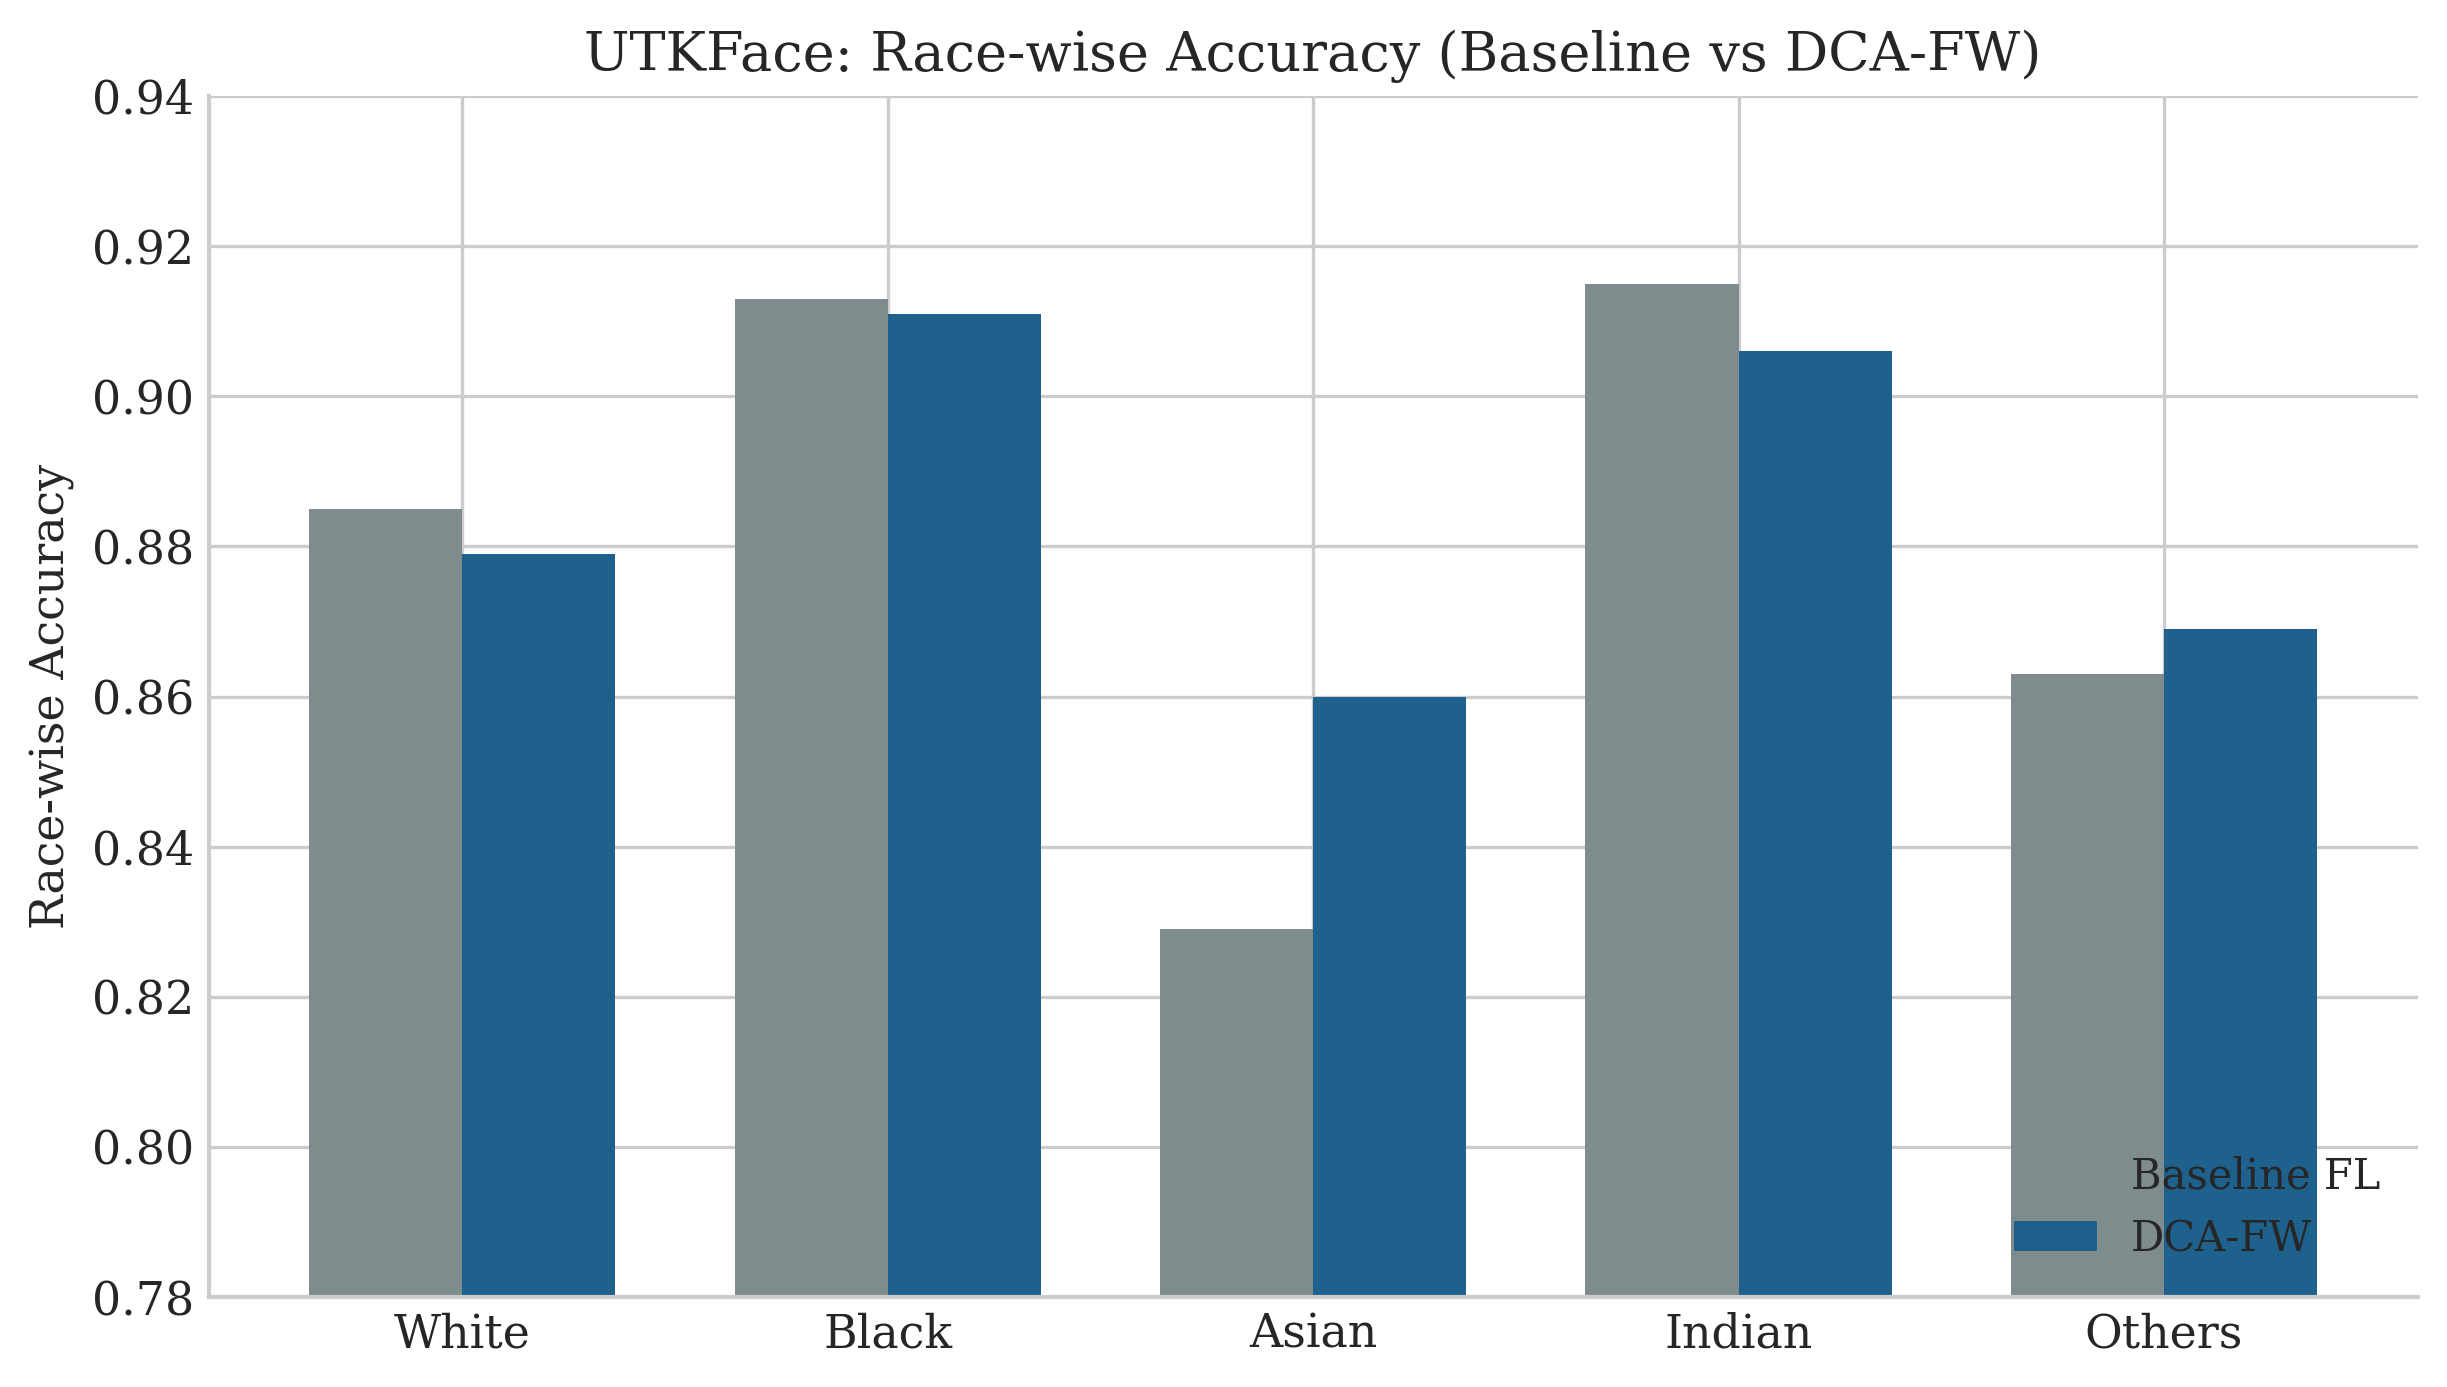
\includegraphics[width=0.88\textwidth]{plots/fig_utk_racewise_baseline_vs_dcafw.png}
\caption{UTKFace race-wise accuracy: baseline FL versus DCA-FW.}
\end{figure}

\begin{figure}[H]
\centering
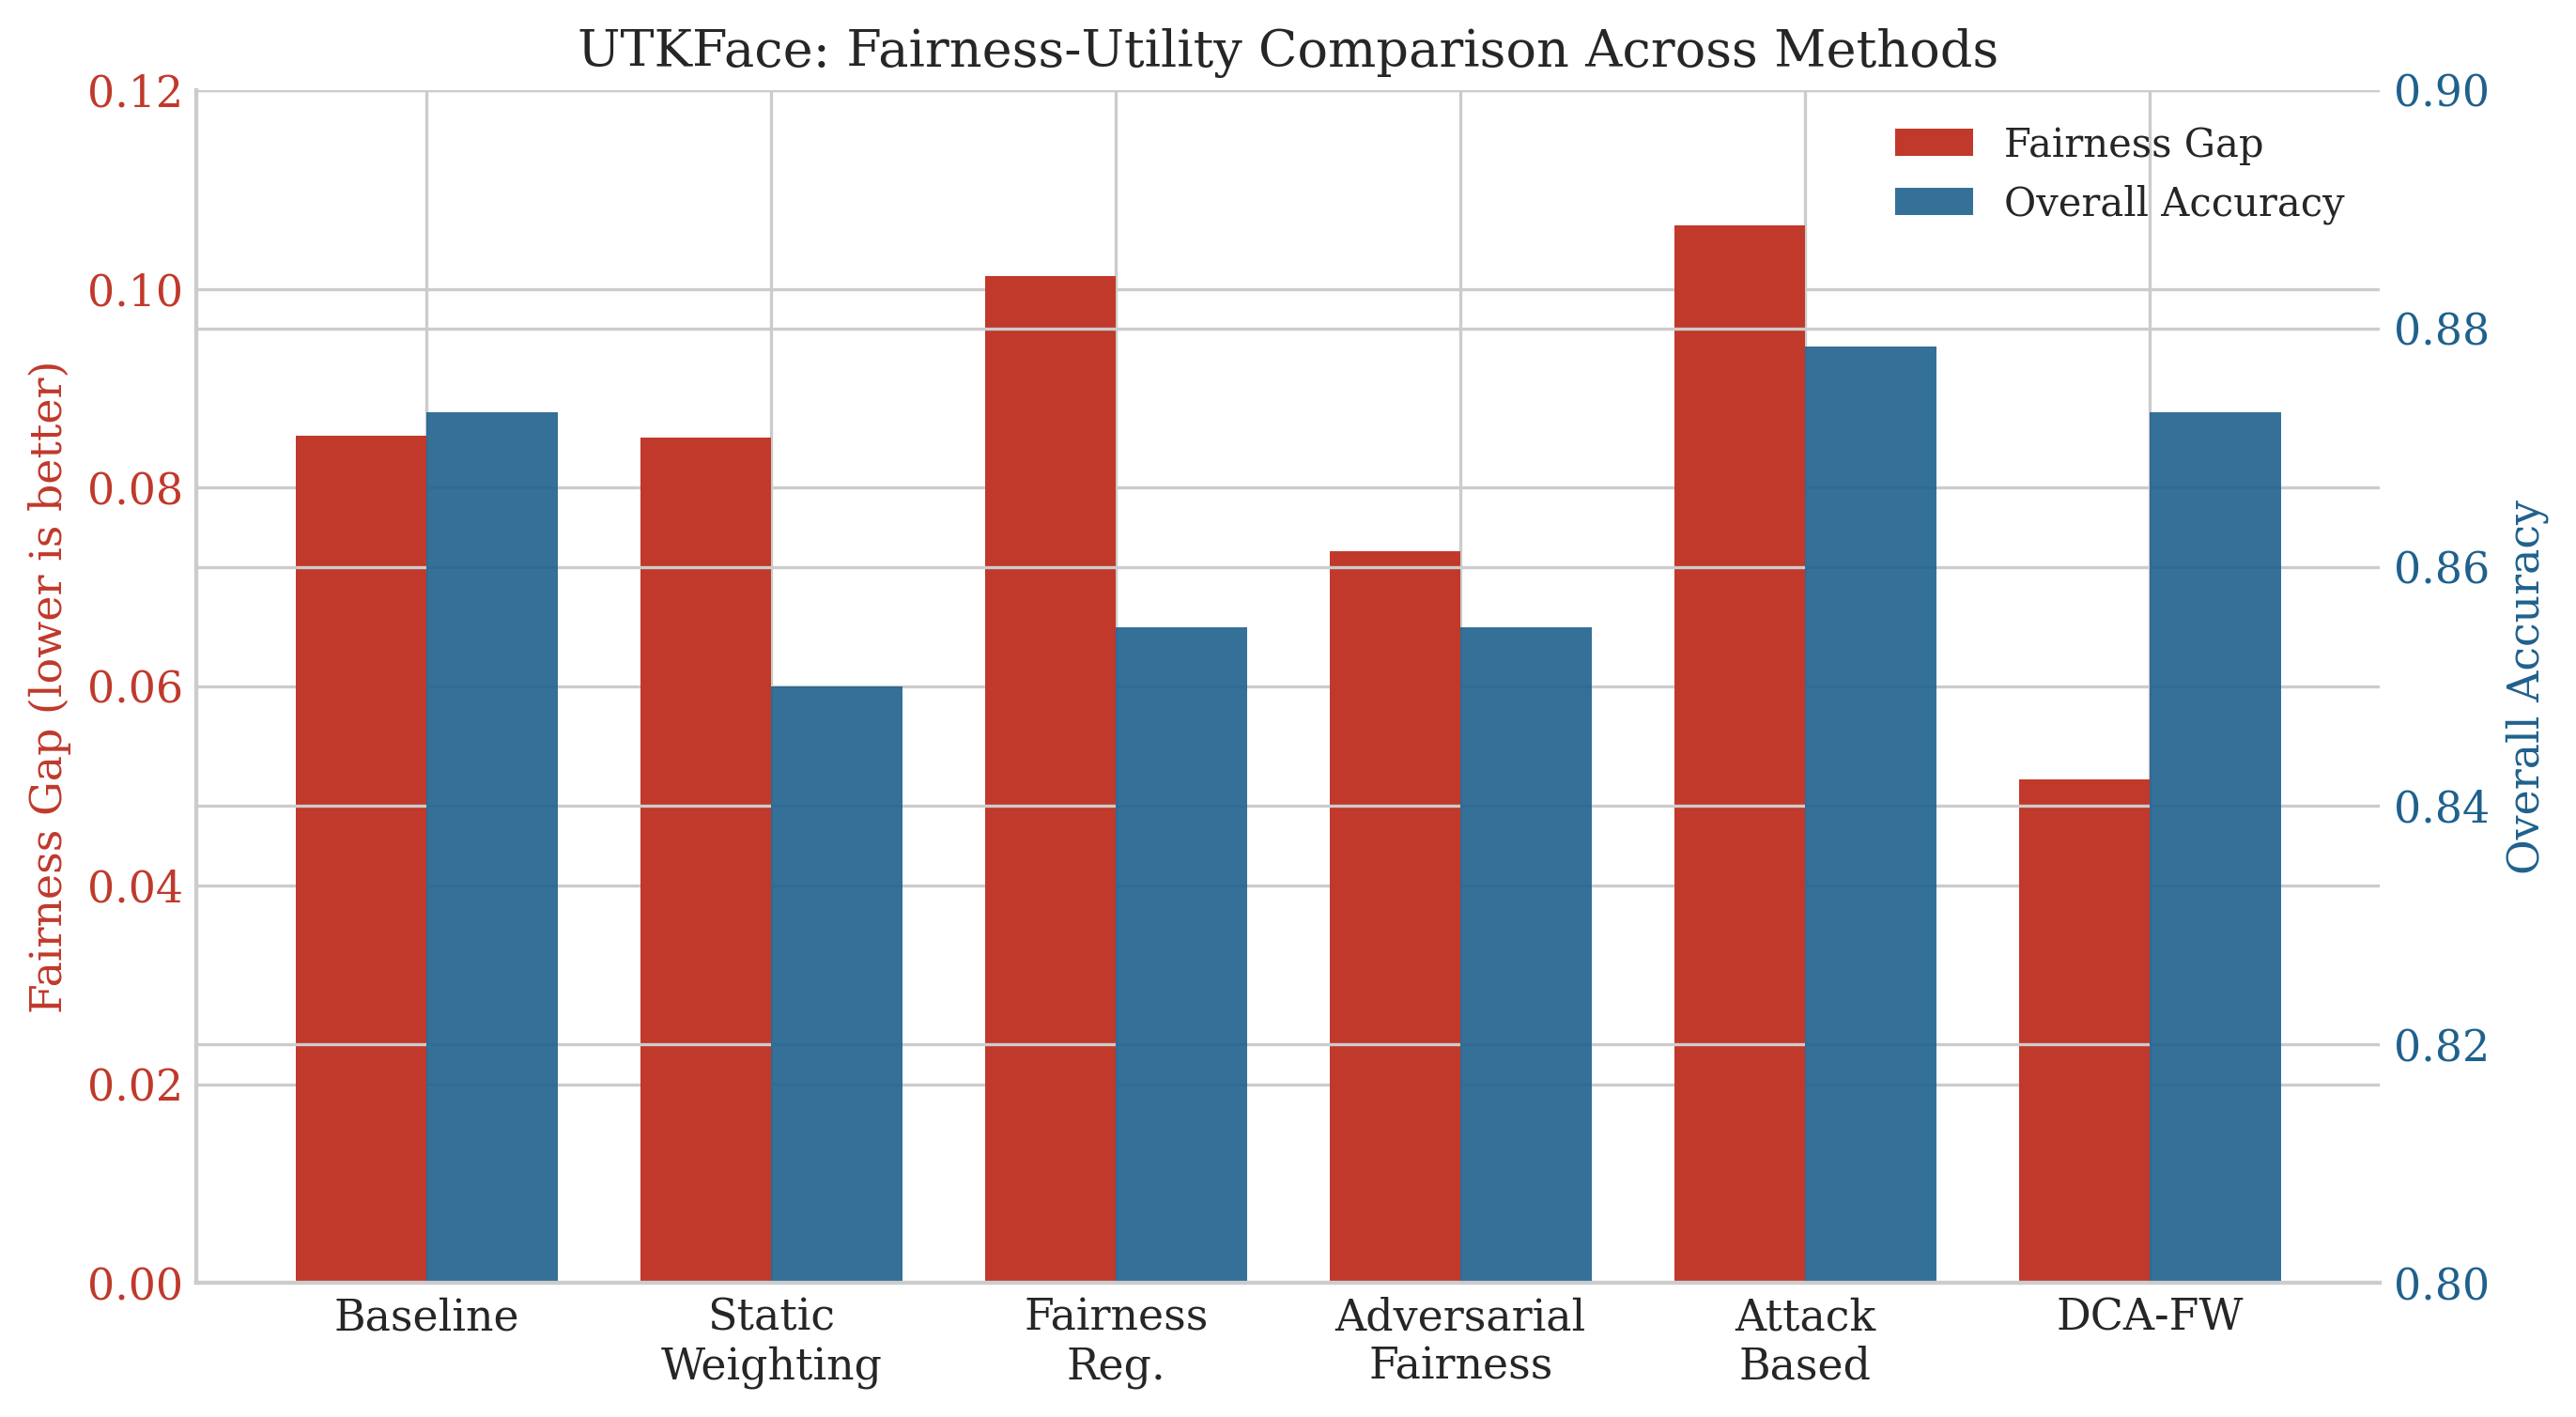
\includegraphics[width=0.88\textwidth]{plots/fig_utk_method_gap_accuracy.png}
\caption{UTKFace method-level fairness-utility comparison.}
\end{figure}

\subsection{Method-Level Interpretation}
Static weighting and fairness regularization did not provide robust gains under FL aggregation. Adversarial fairness learning improved fairness moderately but introduced optimization overhead and slight utility reduction. The attack-based strategy failed as a constructive fairness mechanism. DCA-FW remained the most effective because its fairness signal is local, adaptive, and aligned with the source of client-level imbalance.

\begin{table}[H]
\centering
\small
\begin{tabular}{lcc}
\toprule
\textbf{Method} & \textbf{Fairness Gap} & \textbf{Overall Accuracy} \\
\midrule
Baseline FL & 0.0852 & 0.873 \\
Static weighting & $\approx 0.085$ & 0.845--0.855 \\
Fairness regularization & 0.1013 & 0.850--0.860 \\
Adversarial fairness & 0.0736 & 0.850--0.860 \\
Attack-based intervention & 0.1064 & 0.873--0.884 \\
\textbf{DCA-FW} & \textbf{0.0507} & \textbf{0.873} \\
\bottomrule
\end{tabular}
\caption{UTKFace method comparison showing DCA-FW as best fairness-utility trade-off.}
\end{table}

\section{Results on FairFace (Validation)}
\subsection{Cross-Dataset Generalization}
The FairFace evaluation validates whether the intervention transfers across a different demographic composition and data source. The baseline run shows a fairness gap of 0.0992. Across DCA-FW runs with increasing fairness-client participation, fairness gap decreases consistently, while overall accuracy remains within a tight operating band.

\begin{table}[H]
\centering
\small
\begin{tabular}{lcc}
\toprule
\textbf{Setting} & \textbf{Overall Accuracy} & \textbf{Fairness Gap} \\
\midrule
Baseline FL & 0.7723 & 0.0992 \\
DCA-FW Run 1 (40\%) & 0.7790 & 0.0880 \\
DCA-FW Run 2 (50\%) & 0.7695 & 0.0858 \\
DCA-FW Run 3 (60\%) & N/A & 0.0812 \\
\bottomrule
\end{tabular}
\caption{FairFace baseline and DCA-FW results across runs.}
\end{table}

\begin{figure}[H]
\centering
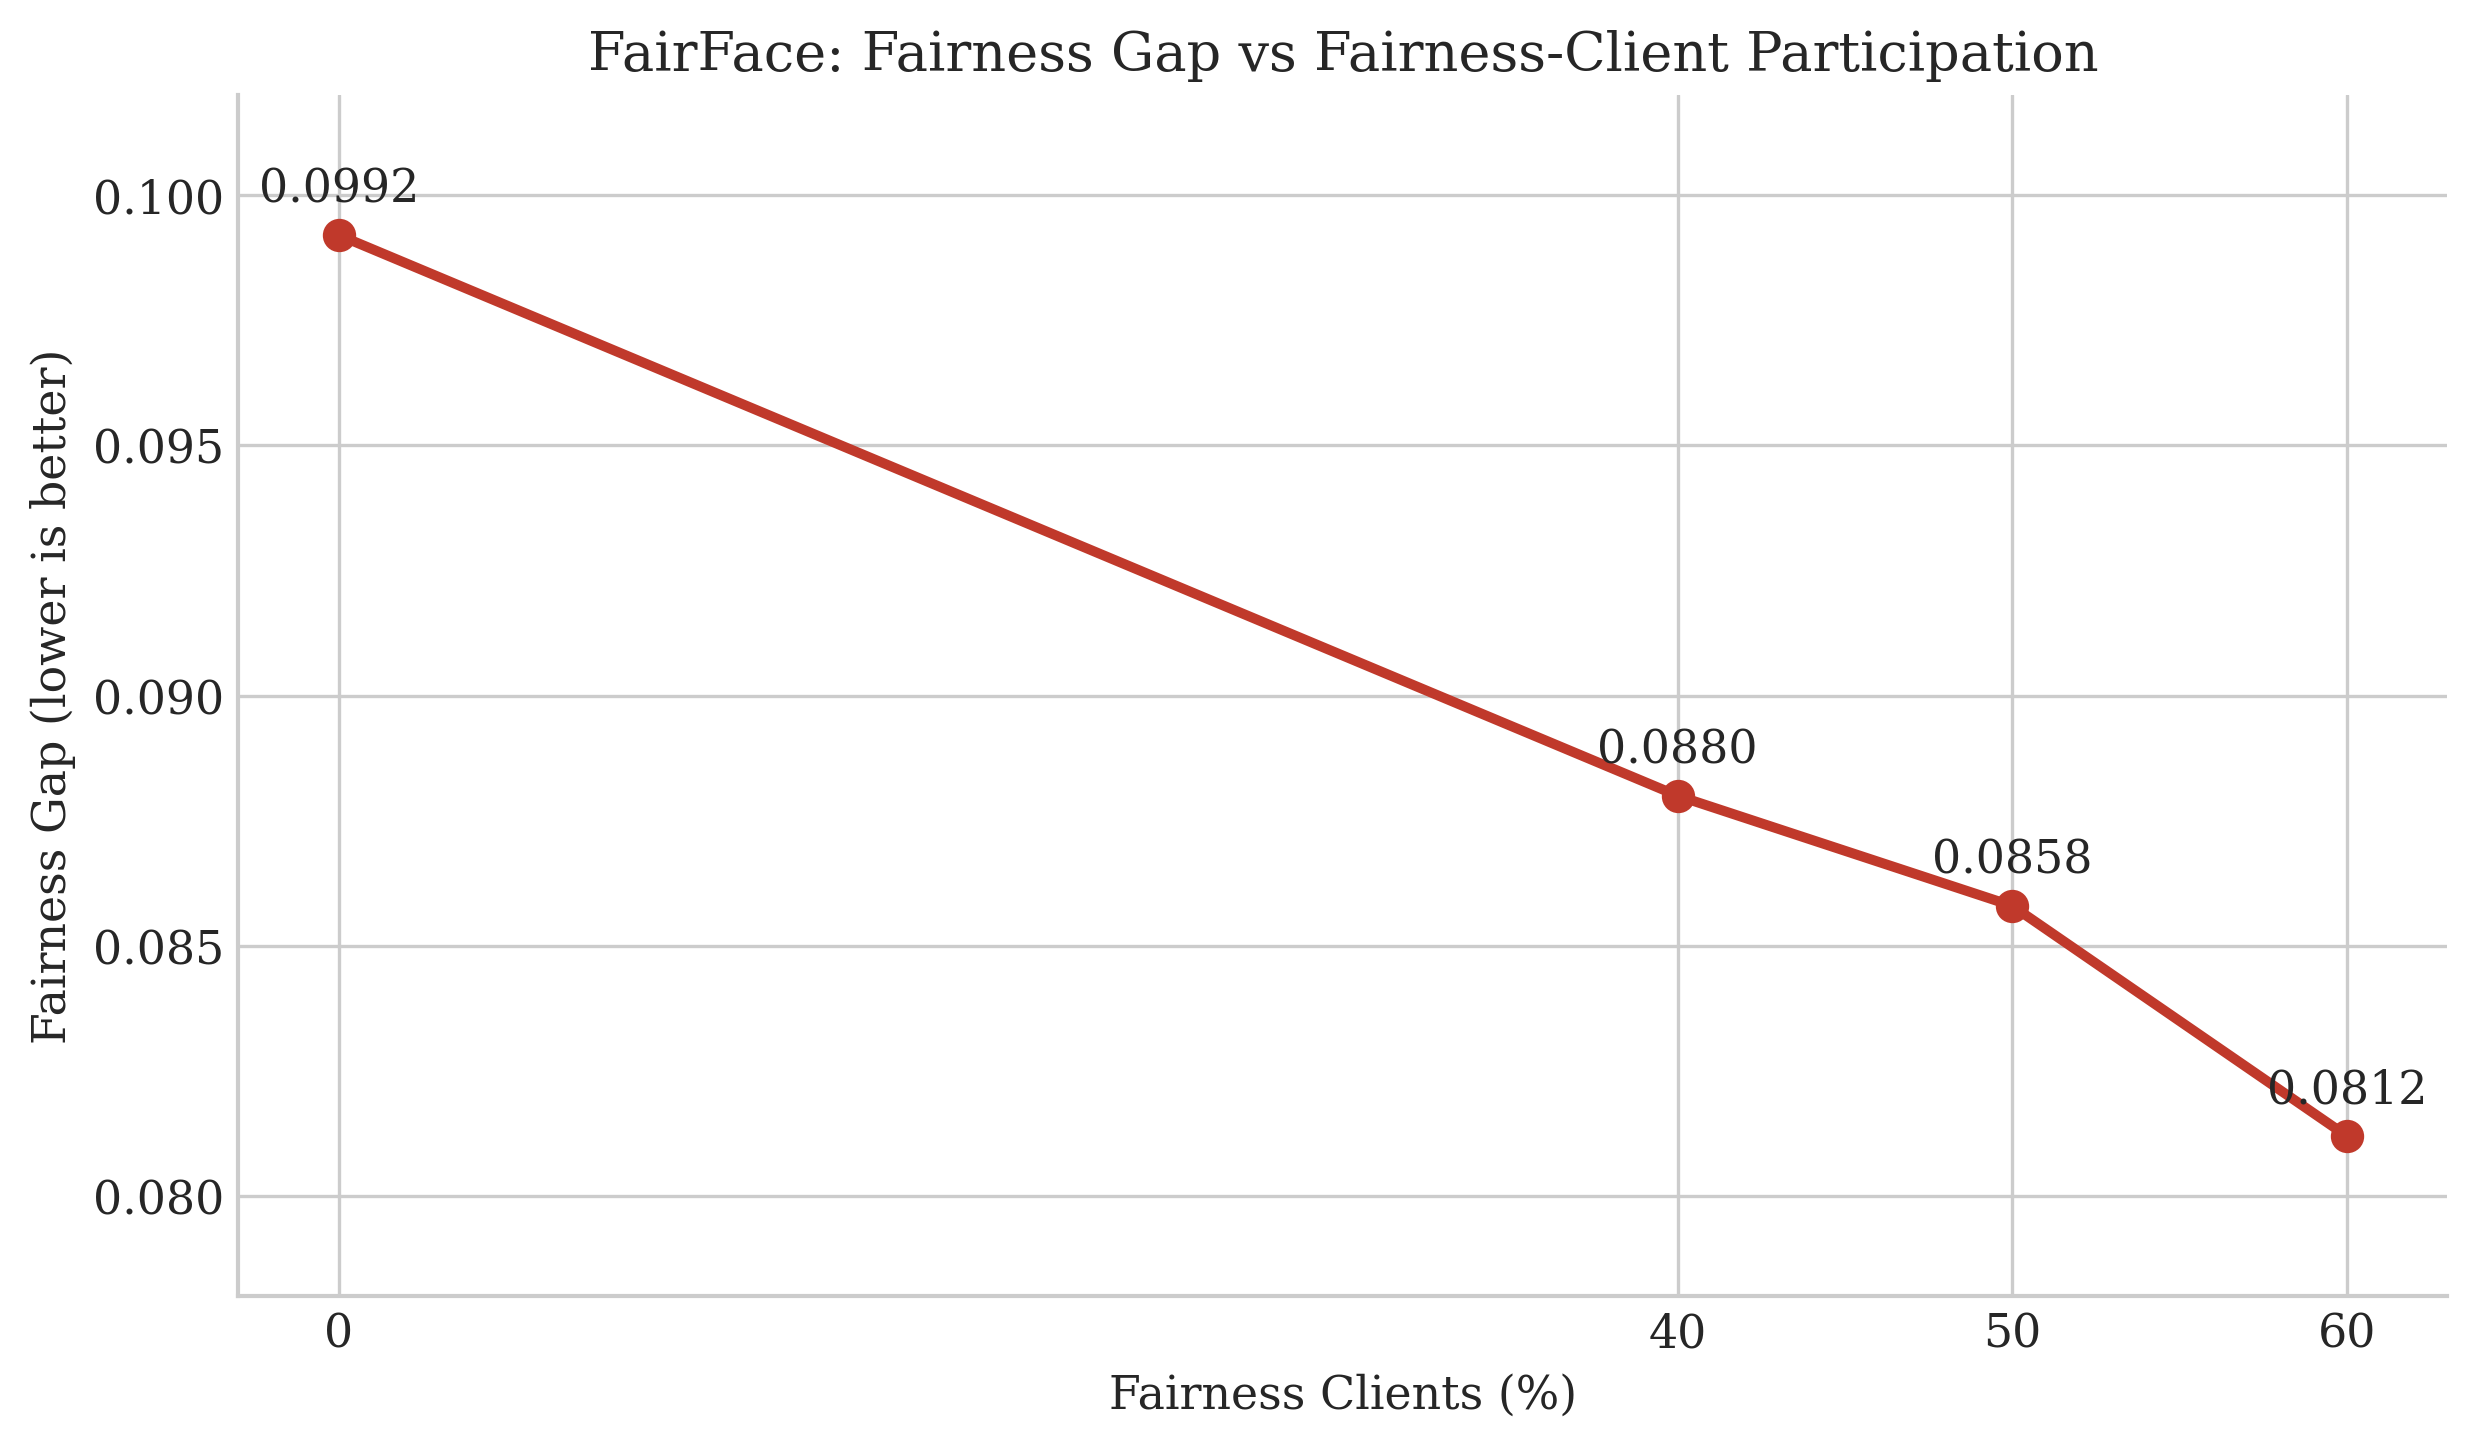
\includegraphics[width=0.88\textwidth]{plots/fig_fairface_gap_vs_fairness_clients.png}
\caption{FairFace fairness gap versus fairness-client participation ratio.}
\end{figure}

\begin{figure}[H]
\centering
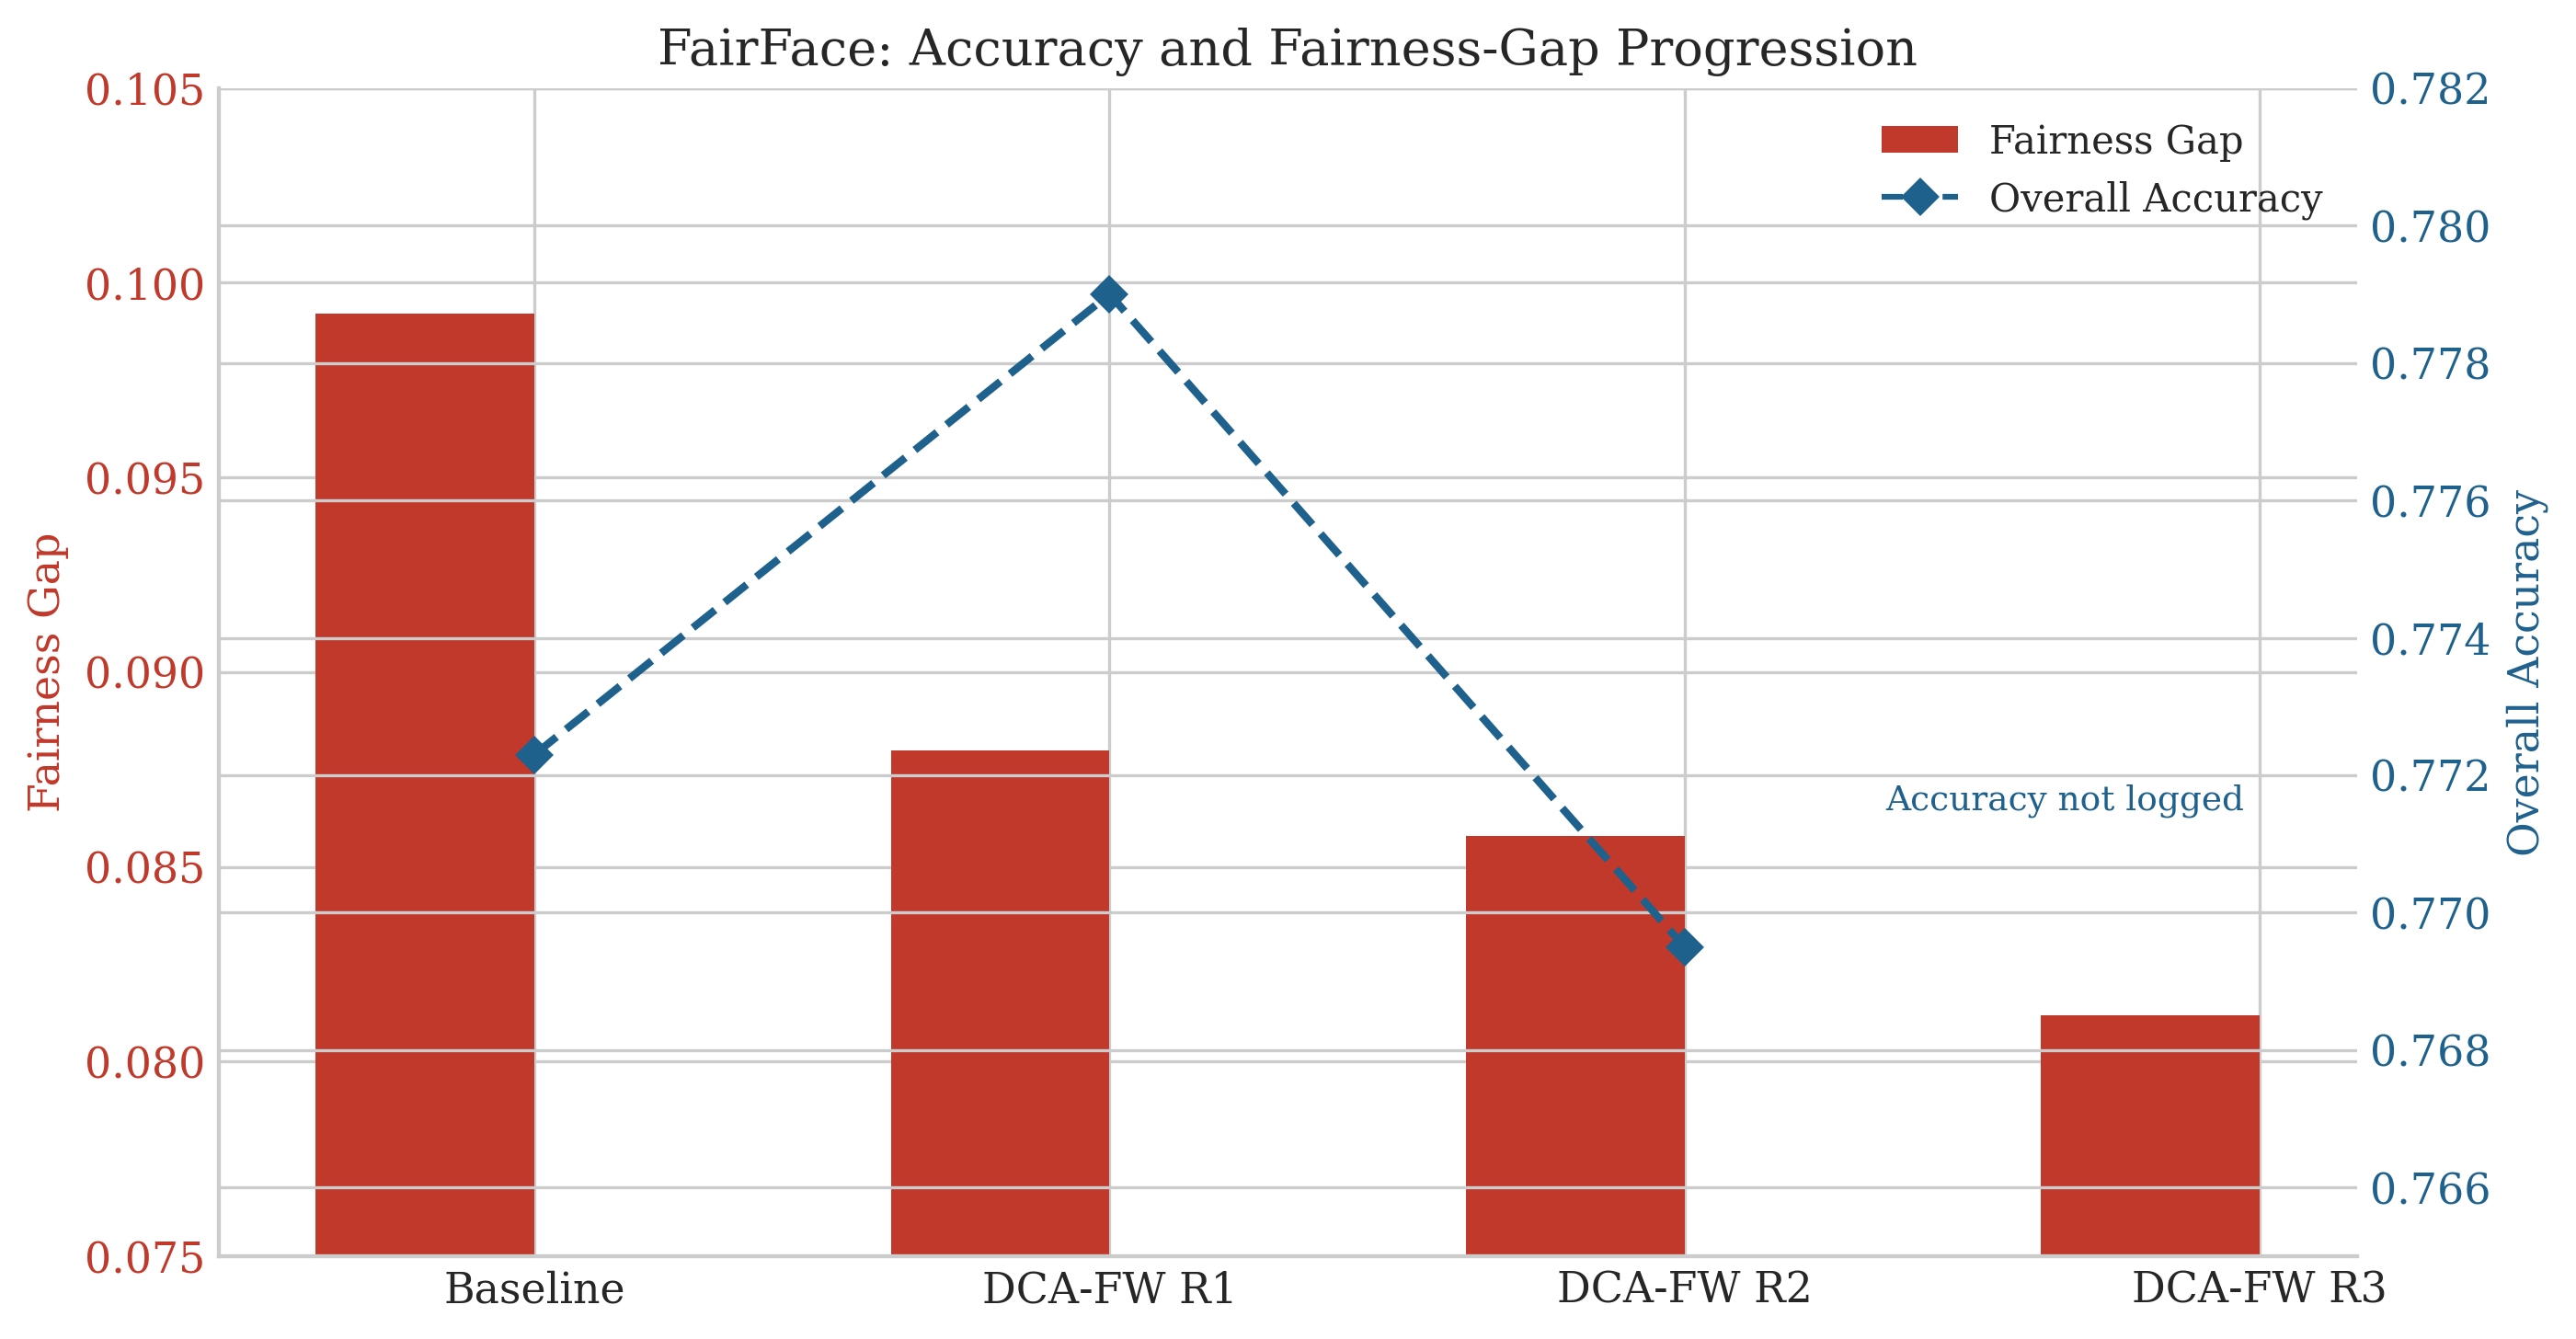
\includegraphics[width=0.88\textwidth]{plots/fig_fairface_accuracy_gap_runs.png}
\caption{FairFace progression of fairness gap and overall accuracy across runs.}
\end{figure}

\begin{figure}[H]
\centering
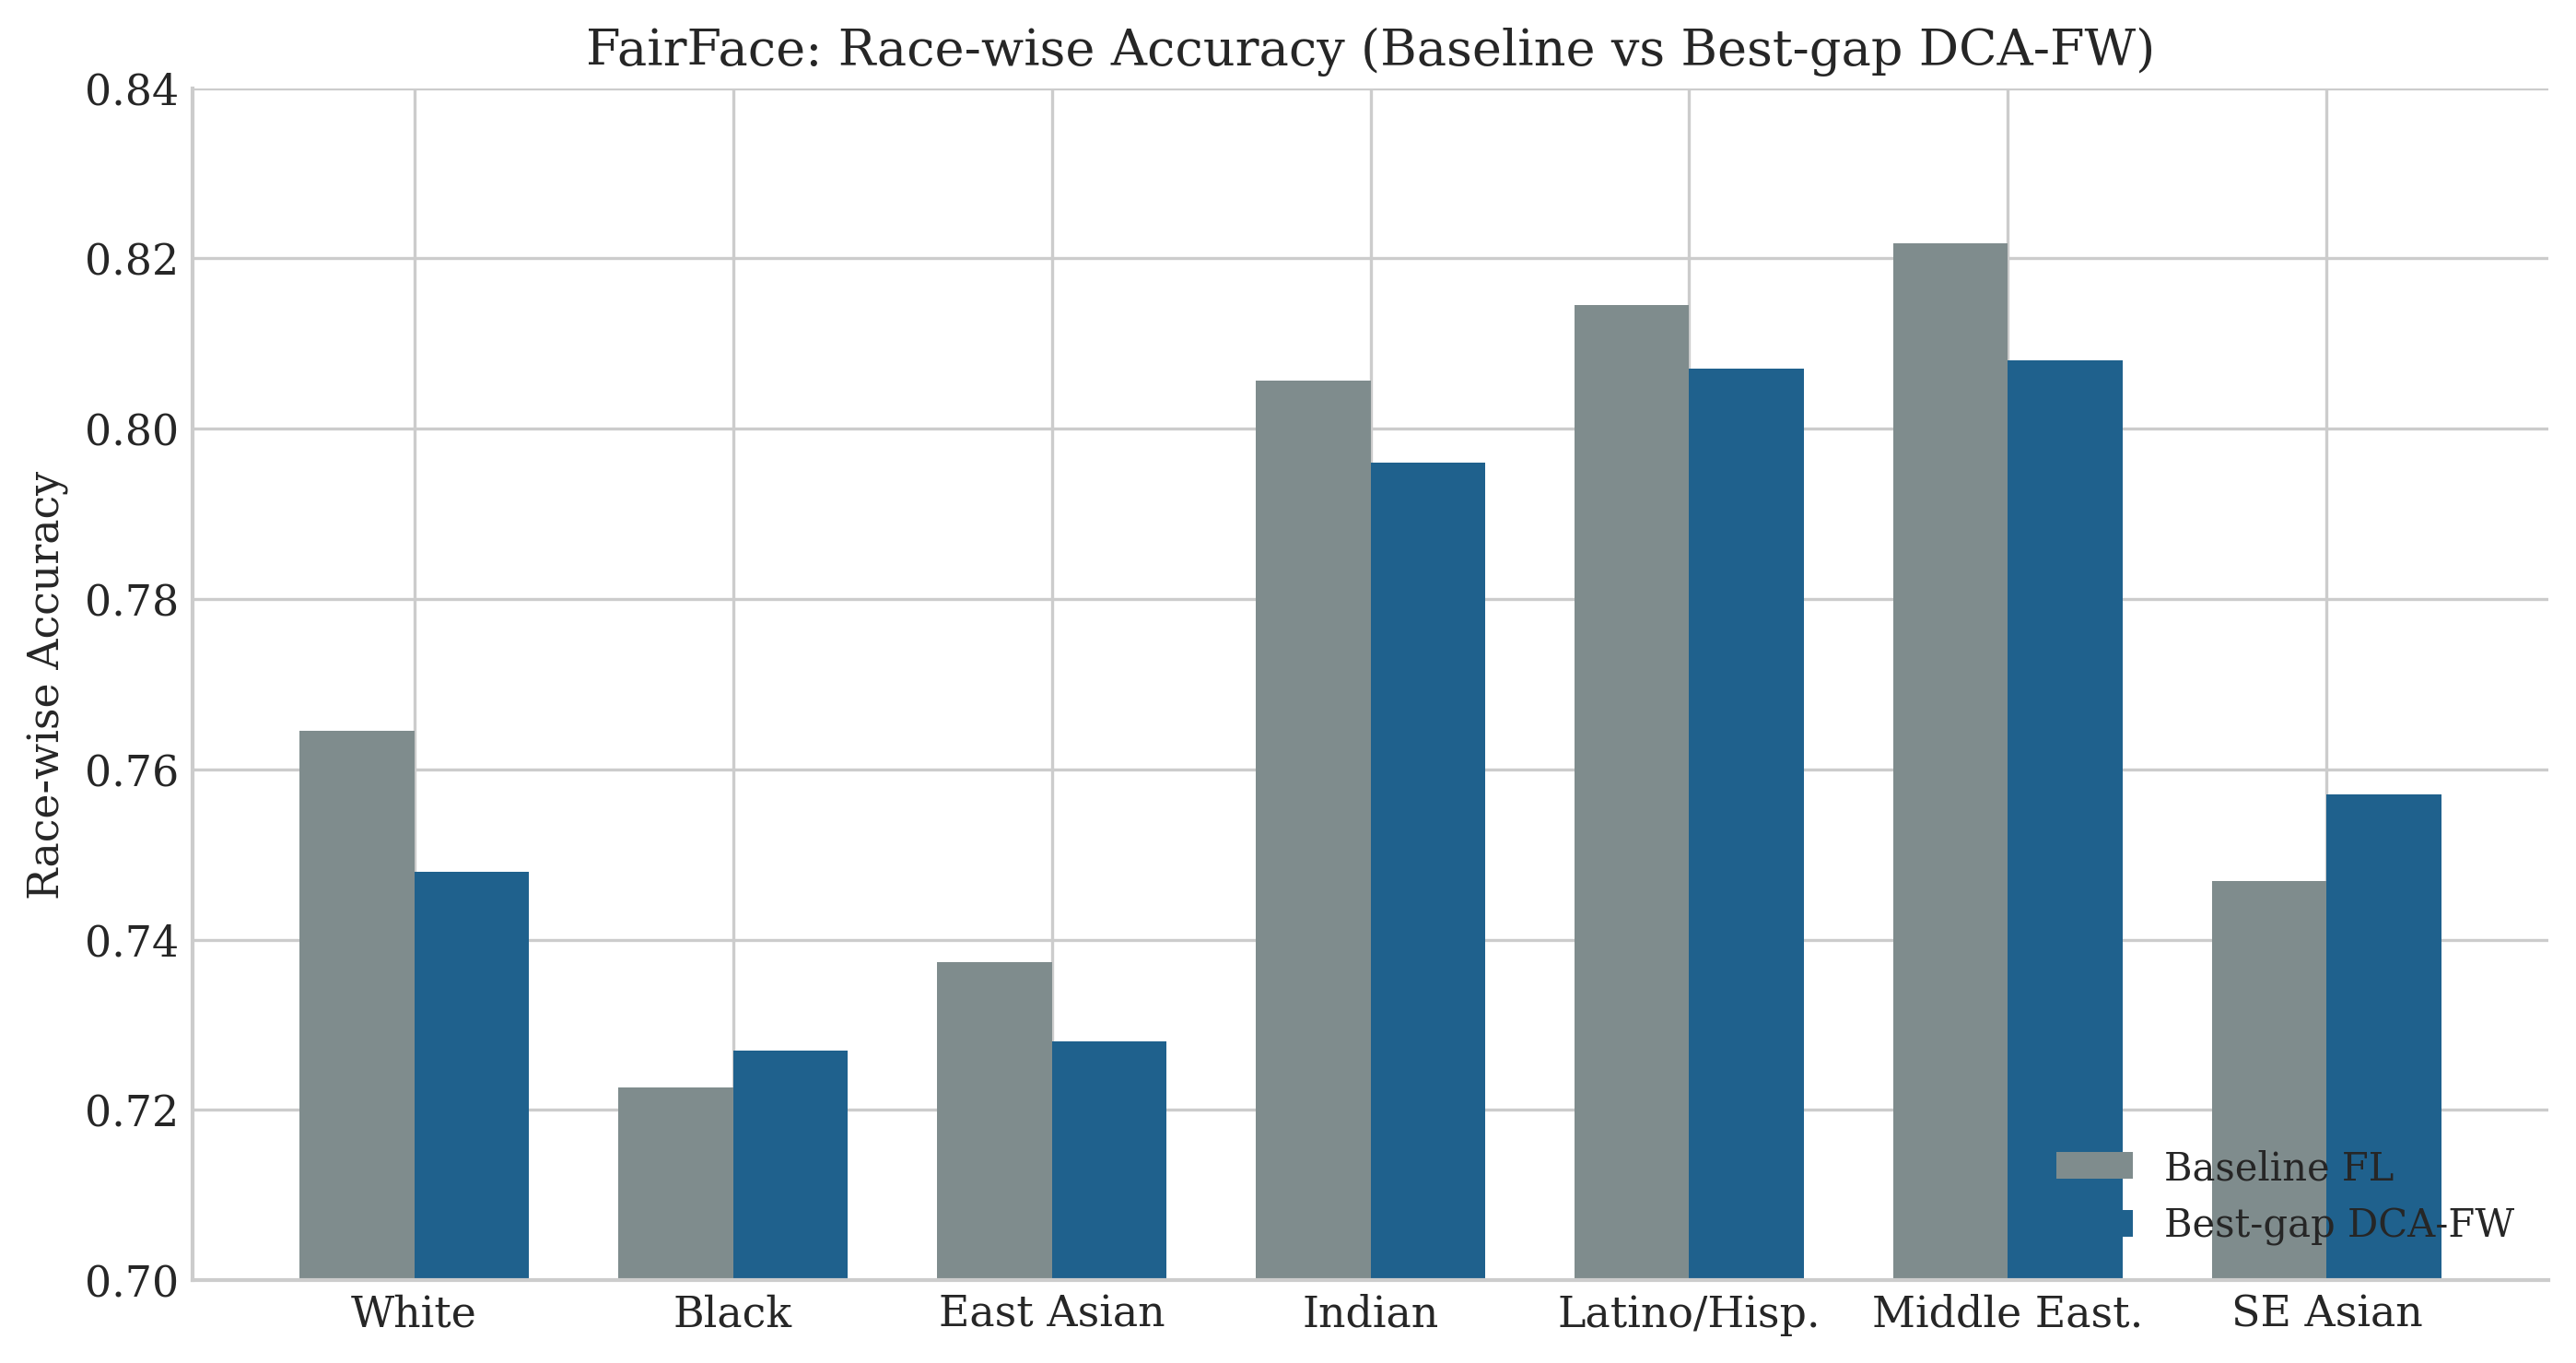
\includegraphics[width=0.88\textwidth]{plots/fig_fairface_racewise_baseline_vs_best_dcafw.png}
\caption{FairFace race-wise accuracy: baseline FL versus best-gap DCA-FW run.}
\end{figure}

\subsection{Validation Summary}
The FairFace trend confirms that DCA-FW is not dataset-specific. Increasing fairness-client participation improves disparity outcomes in a monotonic fashion in the reported runs, and no major utility collapse is observed. This supports the claim that adaptive local weighting is a practical fairness mechanism for decentralized training with heterogeneous client data.

\section{Discussion}
The empirical results indicate that fairness interventions in FL should be placed at the same granularity as data heterogeneity: the client. Global fairness penalties and static weighting provide weak corrective signals after aggregation, particularly when client distributions differ strongly. DCA-FW avoids this mismatch by adjusting group emphasis locally from observed local errors. The method is simple to integrate into existing FL loops, requires no extra model head, and introduces minimal communication overhead.

A practical interpretation is that fairness improvement in FL is an optimization alignment problem. If the corrective signal is generated where disparity appears (local data), and updated at the same cadence as local optimization (per round), fairness gains are stable and utility-preserving.

\section{Limitations and Future Work}
This study focuses on binary gender classification and race-wise evaluation. Future extensions should include multi-label settings, intersectional attributes, and stronger adversarial models (e.g., model poisoning with adaptive objectives). Another useful direction is principled fairness-client scheduling, where client participation is selected dynamically based on per-round contribution estimates. Formal convergence analysis for DCA-FW and robust confidence-interval reporting over multiple seeds are also important next steps.

\section{Conclusion}
This work demonstrates that standard federated training can retain high global accuracy while exhibiting meaningful demographic disparity. Among evaluated methods, DCA-FW provides the best and most consistent fairness-utility balance. On UTKFace, fairness gap improves from 0.0852 to 0.0507 with preserved overall accuracy. On FairFace, fairness gap improves from 0.0992 to 0.0812 across adaptive runs. The overall evidence supports client-adaptive fairness weighting as a strong baseline for practical fairness-aware federated learning systems.

\section*{References}
\addcontentsline{toc}{section}{References}
\begin{enumerate}
    \item McMahan, B., Moore, E., Ramage, D., Hampson, S., and Arcas, B. A. y. (2017). Communication-Efficient Learning of Deep Networks from Decentralized Data. \textit{AISTATS}.
    \item Kairouz, P. et al. (2021). Advances and Open Problems in Federated Learning. \textit{Foundations and Trends in Machine Learning}, 14(1--2), 1--210.
    \item Hardt, M., Price, E., and Srebro, N. (2016). Equality of Opportunity in Supervised Learning. \textit{NeurIPS}.
    \item Zafar, M. B., Valera, I., Gomez-Rodriguez, M., and Gummadi, K. P. (2017). Fairness Constraints: Mechanisms for Fair Classification. \textit{AISTATS}.
    \item Zhang, B. H., Lemoine, B., and Mitchell, M. (2018). Mitigating Unwanted Biases with Adversarial Learning. \textit{AIES}.
    \item Buolamwini, J., and Gebru, T. (2018). Gender Shades: Intersectional Accuracy Disparities in Commercial Gender Classification. \textit{FAT*}.
    \item Karkkainen, K., and Joo, J. (2021). FairFace: Face Attribute Dataset for Balanced Race, Gender, and Age. \textit{WACV}.
    \item Zhang, T. et al. (2020). Fairness and Robustness in Federated Learning. \textit{arXiv:2012.02447}.
\end{enumerate}

\end{document}
